\chapter{Project Context and Objectives}
\label{chap:Project_Context_and_Objectives}

\section*{Introduction}
This chapter delineates the foundational context of the project, elucidates the specific challenges it seeks to address, and establishes the primary objectives that will guide the development of the proposed LegalTech platform.

\section{General Project Framework}

\subsection{General Context}
The contemporary global landscape is characterized by a rapid acceleration in digital transformation, presenting unprecedented opportunities to automate and optimize diverse sectors. However, the legal and administrative domain—particularly within Morocco—remains heavily reliant on traditional, manual methodologies. This pervasive reliance on legacy systems renders the acquisition of accurate legal information and the execution of administrative consultations inherently complex, financially burdensome, and highly resource-intensive.

As first-year engineering students enrolled in the "Advanced Software Engineering for Digital Services" (ASEDS) program at the National Institute of Posts and Telecommunications (INPT), we have cultivated a robust academic foundation encompassing software engineering principles, advanced database management, and the architecture of complex digital systems \cite{ref2}. Capitalizing on this foundation and the ongoing revolution in artificial intelligence, we identified a compelling opportunity to harness these emerging technologies. By focusing specifically on the LegalTech domain, we aim to modernize this critical sector, facilitating seamless, reliable, and democratized access to legal information for the general public.

\subsection{Problem Statement}
Despite the pressing need to digitize the legal sector, the integration of artificial intelligence into the Moroccan legal framework encounters several distinct technical and economic hurdles. These challenges can be synthesized as follows:

\begin{itemize}
    \item \textbf{Prohibitive Costs and Automation Deficits:} The systemic lack of automation in the legal sector renders professional consultations prohibitively expensive. Legal consultants typically mandate substantial fees, presenting the average user with a severe dilemma: either expend inordinate hours conducting manual, often fruitless web searches, or incur exorbitant costs for a fundamental legal inquiry.
    
    \item \textbf{Limitations of Global LLMs (The Hallucination Risk):} Despite the extraordinary capabilities of Large Language Models (LLMs), these architectures are predominantly trained on foreign, anglo-centric datasets and inherently lack deep, localized knowledge of Moroccan legal jurisprudence. Consequently, when queried regarding specific Moroccan legal procedures, these models frequently succumb to "hallucinations," generating confident but entirely fabricated and factually incorrect responses.
    
    \item \textbf{Data Extraction Bottlenecks (Unstructured Document Formats):} Moroccan legal documents and administrative circulars are rarely distributed in machine-readable, digital-native formats. Instead, they predominantly exist as scanned, image-based PDF files replete with complex tabular matrices, official stamps, and handwritten signatures. Traditional Optical Character Recognition (OCR) heuristics consistently fail to process and accurately extract structured semantic data from these artifacts.
    
    \item \textbf{Linguistic and Semantic Barriers:} The vast majority of official documentation is drafted in formal, highly structured Legal Arabic. Processing this specific dialect necessitates a robust, specialized Embedding Model explicitly trained on Arabic semantic structures to execute accurate mathematical vector searches.
\end{itemize}

\subsection{Project Objectives}
In direct response to these multi-faceted challenges, this project endeavors to architect and deploy an integrated digital platform. The successful realization of this platform is predicated on achieving the following primary and secondary objectives:

\begin{itemize}
    \item Conduct a rigorous needs analysis and formally draft a comprehensive project specifications document.
    \item Evaluate and select an optimal, modern technology stack capable of supporting high-performance enterprise requirements.
    \item Architect an advanced Retrieval-Augmented Generation (RAG) system specifically designed to eradicate AI hallucination by forcing the generative model to synthesize answers exclusively from verified Moroccan legal sources.
    \item Implement state-of-the-art OCR pipelines and multilingual Embedding Models to ensure high-fidelity data ingestion.
    \item Develop an intuitive, responsive User Interface (UI) featuring:
    \begin{itemize}
        \item A real-time chat interface allowing users to converse dynamically with the RAG-powered Legal LLM.
        \item A multimodal bypass system empowering users to upload and query their personal documents directly.
        \item A Split-Screen \LaTeX\ Editor enabling users to autonomously draft, modify, and compile professional legal documents via code or through AI-driven template injection.
    \end{itemize}
    \item Implement a robust Identity and Access Management (IAM) system for secure authentication.
    \item Enforce strict data security and Row-Level Security (RLS) policies to protect user metadata and uploaded artifacts.
    \item Design a highly normalized, asynchronous relational database.
    \item Engineer a comprehensive, JSON-based telemetry and logging system to monitor backend execution and AI latencies.
    \item Optimize backend concurrency to support high-volume parallel requests while minimizing operational cloud costs.
    \item Execute exhaustive Quality Assurance (QA) and end-to-end testing protocols to guarantee systemic stability.
    \item Finalize and execute the production deployment of the platform.
\end{itemize}

\newpage
\section{Project Management and Methodology}

\subsection{Adopted Methodology}

\subsubsection{The Scrum Framework}
Scrum is an agile organizational framework utilized to manage the development of complex products. Defined by its creators as an iterative, holistic framework, Scrum focuses on achieving common objectives by delivering high-value products in a productive and creative manner. It is widely recognized as a premier implementation of the Agile Manifesto's core principles.

\begin{figure}[htbp]
    \centering
    \IfFileExists{Figures/1.jpg}{
        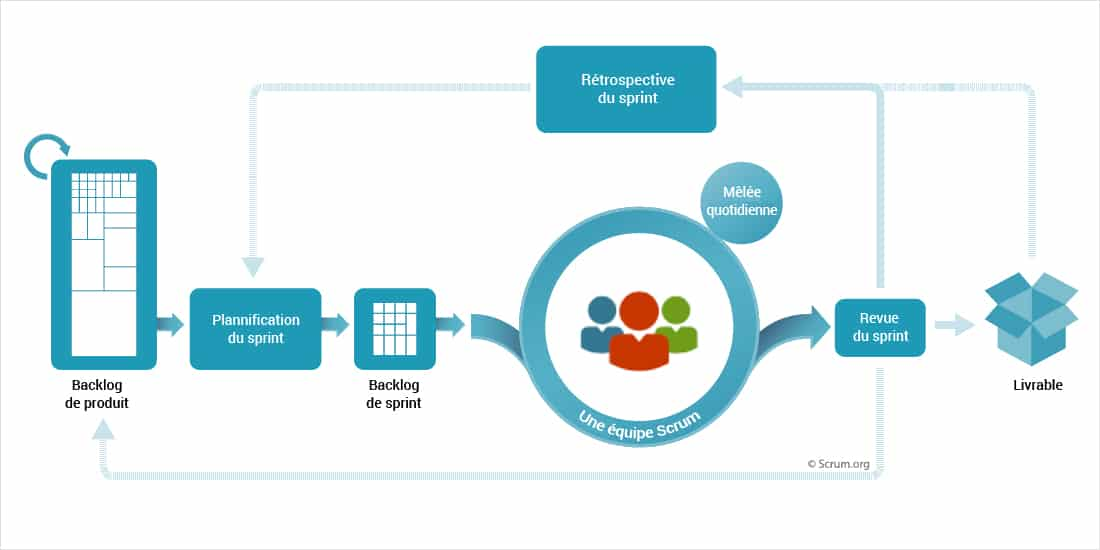
\includegraphics[width=0.85\textwidth, keepaspectratio]{Figures/1.jpg}
    }{
        \framebox[0.85\textwidth]{\rule{0pt}{150pt} \textbf{Missing Image: Figures/1.jpg}}
    }
    \caption{Visual representation of the Scrum Agile methodology.}
    \label{fig:scrum_schema}
\end{figure}

Implementing a project under Scrum best practices requires the following foundational elements:
\begin{itemize}
    \item An autonomous, highly responsible cross-functional team capable of rapidly adapting to dynamic client requirements or pivoting technical scopes.
    \item A structural workflow organized into "Sprints": short, time-boxed iterations (typically 2 to 4 weeks) facilitating rapid intervention and continuous integration.
    \item A rigorous definition of requirements, systematically consolidated into an evolving master task list known as the "Product Backlog."
\end{itemize}

\subsubsection{Roles within Scrum}
The Scrum framework prescribes three primary roles:
\begin{enumerate}[label=\arabic*)]
    \item \textbf{The Product Owner:} The product's visionary and the primary proxy for the client's expectations. This role mandates high availability to resolve ambiguities and prioritize the backlog.
    \item \textbf{The Scrum Master:} The facilitator responsible for ensuring absolute adherence to Scrum values. The Scrum Master shields the team from external disruptions and orchestrates the removal of developmental bottlenecks.
    \item \textbf{The Development Team:} A self-managing, autonomous collective devoid of internal hierarchical structures, where technical decisions are deliberated and executed collaboratively.
\end{enumerate}

These entities synergize to execute the following core Scrum events:
\begin{itemize}
    \item \textbf{The Sprint:} A strict time-box defining the developmental cycle.
    \item \textbf{Sprint Planning:} The initial event where the team collaboratively selects specific User Stories from the Product Backlog to target during the impending Sprint.
    \item \textbf{Sprint Execution:} The active developmental phase, encompassing architectural design, programming, and testing.
    \item \textbf{Sprint Review and Retrospective:} The concluding evaluation where the team demonstrates the newly implemented features and introspects on workflow improvements for subsequent Sprints.
    \item \textbf{Backlog Grooming:} The continuous refinement and re-prioritization of the Product Backlog to accommodate shifting project dynamics.
\end{itemize}

\subsection{Role Distribution within the Team}
Given the streamlined nature of our academic development team for this project, the allocation of a dedicated, full-time Scrum Master was structurally impractical. Consequently, we adopted an adapted, highly collaborative Scrum paradigm, dynamically distributing the responsibilities of the Product Owner, Scrum Master, and Developers amongst ourselves to best simulate enterprise Agile workflows.

\subsection{Collaboration and Communication Tools}

\subsubsection{Instant Communication}
We utilized direct messaging platforms (such as WhatsApp) as our primary conduit for rapid coordination, conducting four distinct types of Agile meetings:
\begin{itemize}
    \item \textbf{Daily Stand-ups:} Brief syncs allowing team members to report progress, highlight immediate goals, and flag technical blockers.
    \item \textbf{Pair-Programming Syncs:} Technical deep-dives utilized for complex architectural design and collaborative debugging sessions.
    \item \textbf{Product Demonstration Reviews:} Milestone meetings dedicated to showcasing compiled features and reviewing the project's holistic functionality prior to final delivery.
\end{itemize}

\begin{figure}[htbp]
    \centering
    \IfFileExists{Figures/2.png}{
        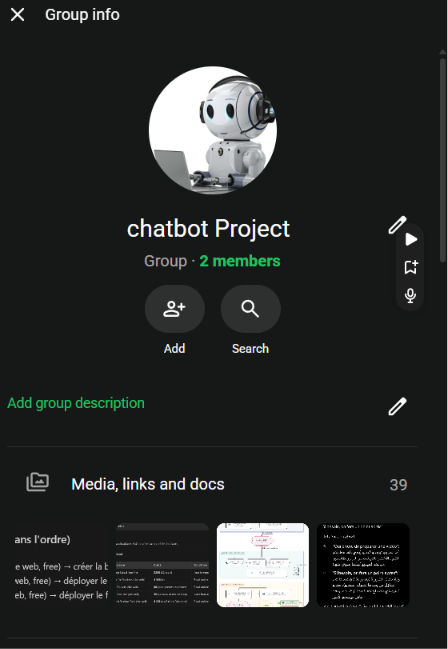
\includegraphics[width=0.4\textwidth, keepaspectratio]{Figures/2.png}
    }{
        \framebox[0.4\textwidth]{\rule{0pt}{100pt} \textbf{Missing Image: Figures/2.png}}
    }
    \caption{Example of team communication and daily stand-ups.}
    \label{fig:communication}
\end{figure}

\subsubsection{Version Control and Source Management}
We strictly enforced version control methodologies utilizing \textbf{Git} and \textbf{GitHub}. This centralized approach guaranteed that the entire team maintained synchronized access to the latest verified codebase. 

We adopted a strict \textbf{Branching and Merging} strategy, ensuring features were isolated during development and only merged into the main production branch following rigorous peer review. Furthermore, every \textbf{Commit} was carefully documented with descriptive syntax, ensuring absolute traceability of the platform's evolutionary history, as illustrated below.

\begin{figure}[htbp]
    \centering
    \IfFileExists{Figures/3.png}{
        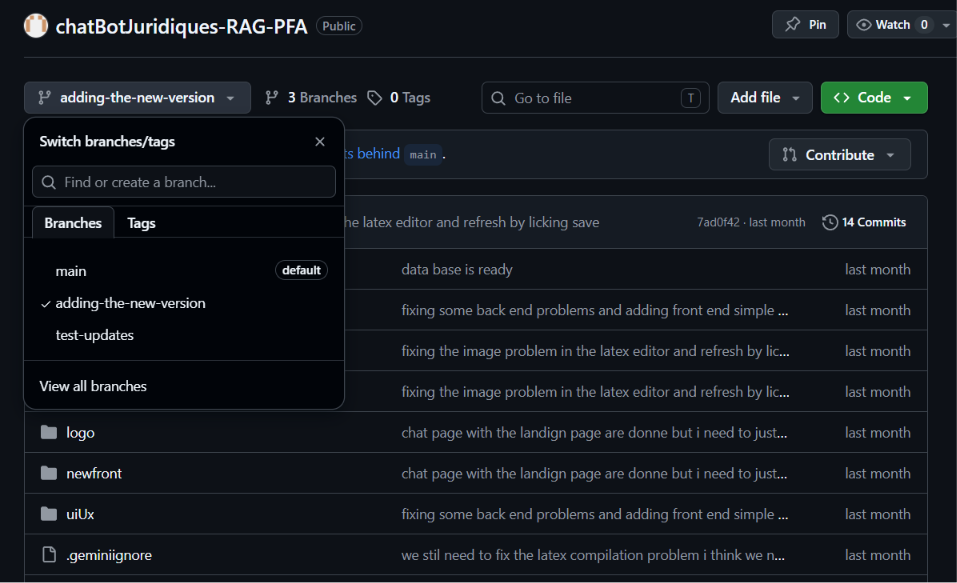
\includegraphics[width=0.9\textwidth, keepaspectratio]{Figures/3.png}
    }{
        \framebox[0.9\textwidth]{\rule{0pt}{150pt} \textbf{Missing Image: Figures/3.png}}
    }
    \caption{Version control trace highlighting Git commits and branches on GitHub.}
    \label{fig:github_commits}
\end{figure}

\section*{Conclusion}
Having firmly established the systemic context, diagnosed the core industry bottlenecks, and articulated the definitive objectives required for project success, the theoretical framework of the LegalTech platform is complete. The subsequent chapters will detail the precise needs specification, the system modeling, and the highly optimized architectural design required to materialize this vision.